\vspace*{4cm}
\part{Messresultate Mesh Benchmark}\label{part:MessresultateMeshBenchmark}
\vspace*{\fill}
\clearpage

\section{Messresultate}\label{sec:Messresultate}
Bei der Durchführung der Mesh Benchmark Messungen wurde für jede Messung unter den entsprechenden Bedingungen ein Messprotokoll resp. eine Auswertung erstellt. Die 8 unterschiedlichen Bedingungen sind in Tabelle \ref{tab:MessungenMeshBenchmark} nochmals zusammengefasst sind.
Diese detaillierten Auswertungen sind im Anhang \ref{app:MessprotokolleMeshBenchmark} dem Bericht angefügt.
Nachfolgend soll exemplarisch eine dieser Auswertungen erläutert werden um aufzuzeigen was diese darstellen und wie diese gelesen werden können.
Eine Interpretation dieser Messresultate ihm Rahmen eines Vergleichs erfolgt schliesslich im Abschnitt \ref{sec:VergleichMeshNetzwerke}.

\begin{table}[h]
\centering
\begin{tabular}{|c|c|c|c|c|c|} 
\hline
\textbf{\#}  & \textbf{Msg. Gen.}  & \textbf{Duration}  & \textbf{Msg. Cnt.}  & \textbf{Payload }  & \textbf{Disturbance}  \\ 
\hline
1 & Rand & 600s & 60 & Small & No \\ 
\hline
2 & Seq & 600s & 60 & Small & No \\ 
\hline
3 & Rand & 600s & 60 & Large & No \\ 
\hline
4 & Seq & 600s & 60 & Large & No \\ 
\hline
5 & Rand & 600s & 600 & Small & No \\ 
\hline
6 & Rand & 600s & 60 & Small & Yes \\ 
\hline
7 & Seq & 750s & 10 & Small & No \\ 
\hline
8 & Seq & 750s & 10 & Large & No \\
\hline
\end{tabular}
\caption{Messungen Mesh Benchmark}
\label{tab:MessungenMeshBenchmark}
\end{table}


\subsection{Resultate}\label{subsec:Resultate}
Die Messresultate im Anhang \ref{app:MessprotokolleMeshBenchmark} wurden mit den Messindizes 1-8 gemäss Tabelle \ref{tab:MessungenMeshBenchmark}, sowie der entsprechenden Messumgebung (z.B. Wohnung) versehen.
So können die Messungen eindeutig identifiziert werden.
Folgende Einschränkungen müssen dabei jedoch beachtet werden:
Gemäss den Erläuterungen im Abschnitt \ref{subsec:Messreihe} wurden die Messungen 6 - 8 nur im Labor Messaufbau durchgeführt. Von diesen Messungen sind also nur diese Auswertung vorhanden.
Weiter musste bei der Durchführung der Messung 5 festgestellt werden, dass die Resultate unbrauchbar waren.
In der Folge dessen wurde die Auswertung dieser Messung gestrichen. Mehr dazu im Abschnitt  \ref{subsec:Validierung}.


Die Abbildungen \ref{fig:VerteilungderLatenzzeiten} bis \ref{fig:OngoingTransactions} zeigen die Messresultate der Messung 2 in der Messumgebung \textit{Wohnung}. Sie stehen exemplarisch für die Messergebnisse aller Messreihen.
In Abbildung \ref{fig:VerteilungderLatenzzeiten} ist die prozentuale Verteilung der Latenzzeiten pro Hop dargestellt.
In sämtlichen Grafiken werden die Ergebnisse von BT Mesh in blau, jene von Thread in grün und jene von Zigbee in rot dargestellt.
So ist ein direkter Vergleich der Protokolle möglich.
Abbildung \ref{fig:VerteilungderLatenzzeiten} sagt also aus wie viele Nachrichten das Ziel mit einer bestimmten Latenzzeit erreicht haben.
Nachrichten die das Ziel nicht erreicht haben, also Pakete die verloren gegangen sind, werden dabei nicht berücksichtigt.
Im gezeigten Beispiel haben rund 76 Prozent der Nachrichten die im BT Mesh Test versendet wurden das Ziel mit einer maximalen Latenzzeit von 10 Millisekunden erreicht.
Die weitere Verteilung geht bis auf Latenzzeiten von über 300 Millisekunden wobei die Prozentzahl der Nachrichten in diesem Bereich sehr tief ist.
Die Werte für Thread und Zigbee zeigen hingegen eine deutlich schmalere Verteilung der Latenzzeiten.

\begin{figure}[h]
	\centering
	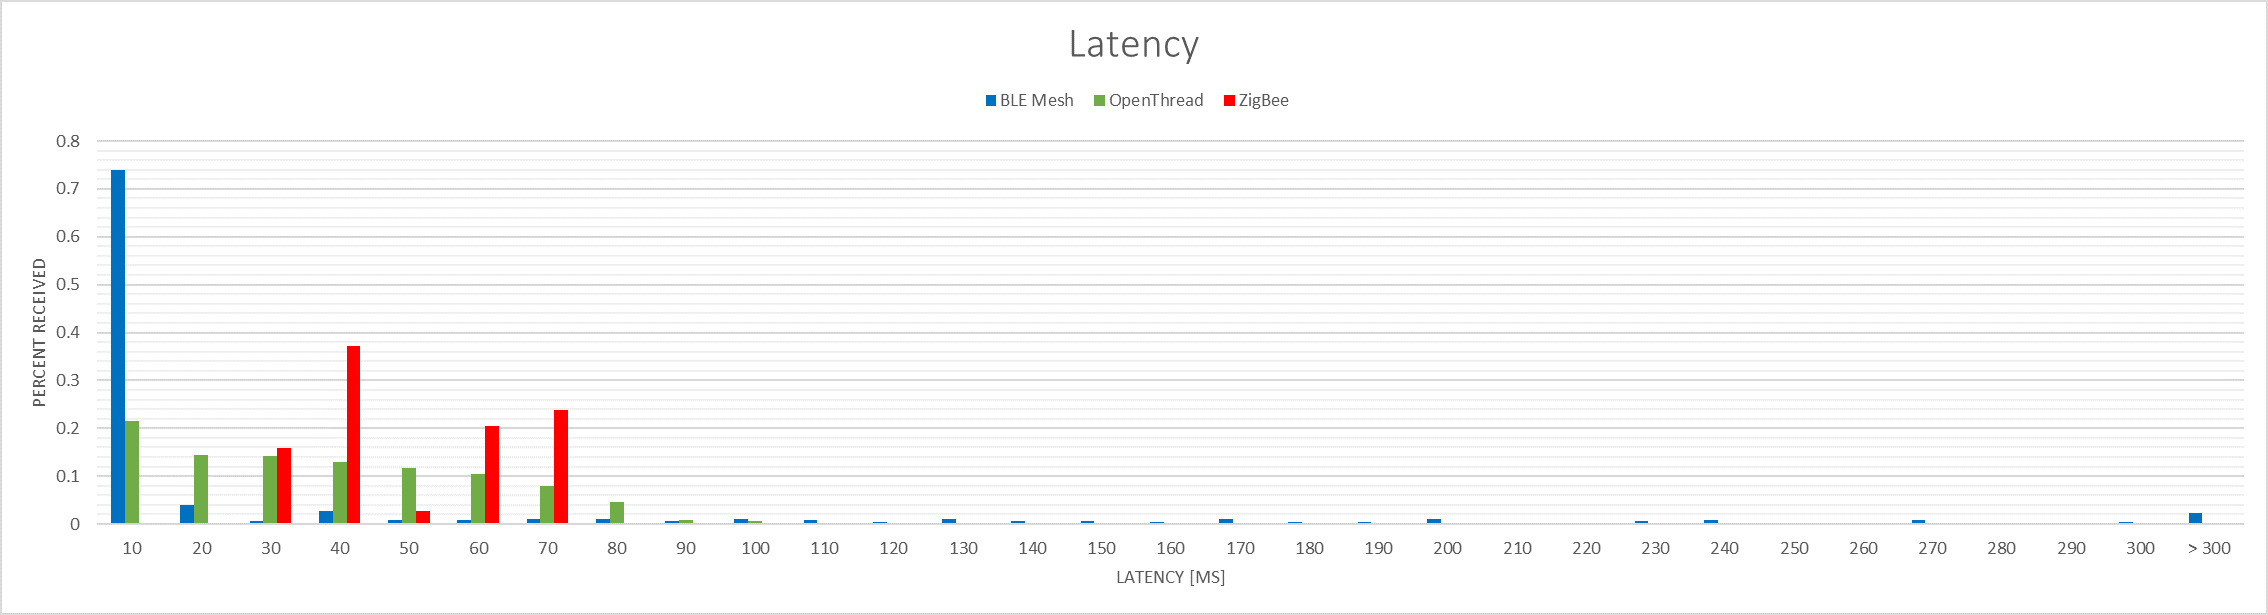
\includegraphics[width=\textwidth]{Latency_2_Wohnung.png}
	\caption{Messung 2 Wohnung: Verteilung der Latenzzeiten pro Hop}
	\label{fig:VerteilungderLatenzzeiten}
\end{figure}

Aus den in Abbildung \ref{fig:VerteilungderLatenzzeiten} aufgezeigten Latenzzeiten wurde der Durchschnitt gebildet und in Abbildung \ref{fig:DurchschnittlicheLatenzzeit} dargestellt.
Es handelt sich dabei wiederum um die Latenzzeit pro Hop. Im Falle von Zigbee ist dies erwähnenswert, da hier die Anzahl Hops nicht ausgelesen werden konnte (siehe Abschnitt \ref{subsubsec:AnzahlHops}) und die Resultate somit mit Vorsicht interpretiert werden müssen. Mehr dazu in der Validierung im Abschnitt \ref{subsec:Validierung}.

Der durchschnittliche Datendurchsatz der mit der Abbildung \ref{fig:DurchschnittlicherDurchsatz} aufgezeigt wird, muss mit der selben Vorsicht betrachtet werden. Denn auch hier werden die Werte pro Hop für die Berechnung verwendet.
Die präsentierten Werte werden errechnet aus der Paketgrösse (Small oder Large) gemäss den Definitionen in Abschnitt \ref{subsec:AllgemeineBenchmarkParameter} und der Latenzzeit des übertragenen Pakets (siehe Gleichung \ref{eq:BerechnungDurchsatz}.
Dabei werden die Werte für den Durchsatz für jedes empfangene Paket berechnet und davon schliesslich der Mittelwert gebildet und in Abbildung \ref{fig:DurchschnittlicherDurchsatz} dargestellt.
Die oben erwähnten Ausreisser bei BT Mesh bewirken nun einen unerwartet hohen Durchsatz bei BT Mesh im Vergleich zu jenem bei Thread welches konstant tiefe Latenzzeiten hat.

\begin{equation}\label{eq:BerechnungDurchsatz}
TP =  \frac{S_{packet} \cdot 8}{t_{lat}}
\end{equation}

\begin{small}
\begin{center}
\begin{tabular}{ll}
$TP$ & Throughput (kBit/s)\\
$S_{packet}$ & Packetsize (Byte)\\
$t_{lat}$ & Latency time (ms)\\
\end{tabular}
\end{center}
\end{small}

\begin{figure}[!htbp]
\centering
\begin{minipage}[b]{0.49\textwidth}
		\centering
		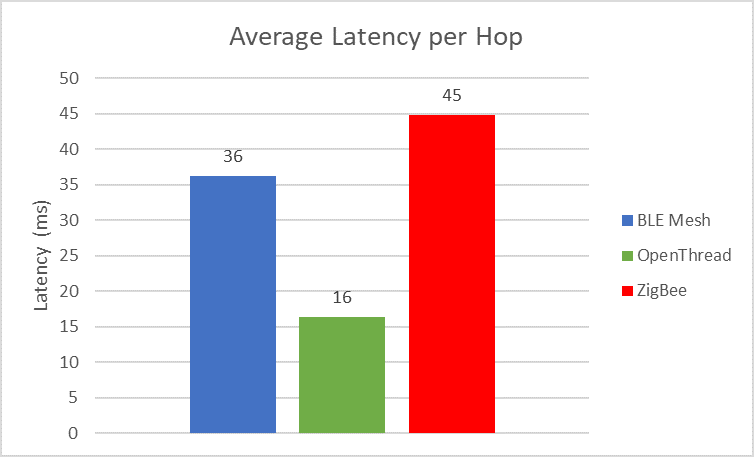
\includegraphics[width=\textwidth]{Average_Latency_per_Hop.png}
		\caption{Messung 2 Wohnung: Durchschnittliche Latenzzeit pro Hop}
		\label{fig:DurchschnittlicheLatenzzeit}
\end{minipage}
\begin{minipage}[b]{0.49\textwidth}
		\centering
		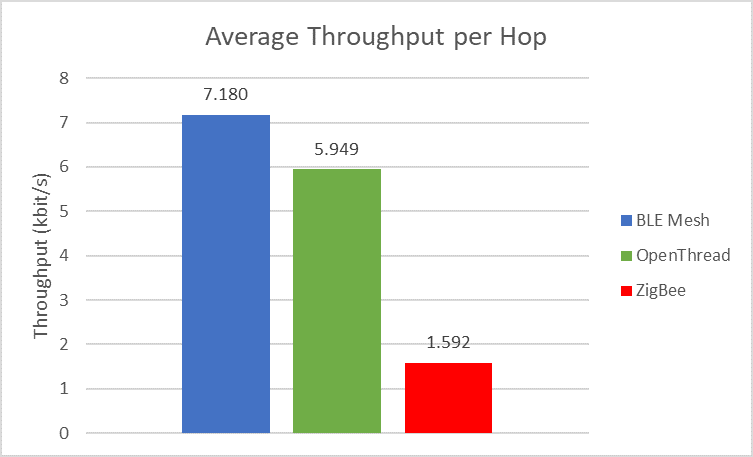
\includegraphics[width=\textwidth]{Average_Throughput_per_Hop.png}
		\caption{Messung 2 Wohnung: Durchschnittlicher Durchsatz pro Hop}
		\label{fig:DurchschnittlicherDurchsatz}
\end{minipage}
\end{figure}

In der Abbildung \ref{fig:DurchschnittlicherPaketverlust} wird der prozentuale Paketverlust gezeigt über die gesamte Anzahl Nachrichten die während dem Benchmark versendet wurden.
Die Paketverluste von einzelnen Client-Server Beziehungen werden nicht separat ausgewertet.
Wiederum im Beispiel von BT Mesh sind in dieser Messung 2.07 \% der Pakete nicht am Ziel angekommen.

\begin{figure}[!htbp]
\centering
\begin{minipage}[b]{0.49\textwidth}
		\centering
		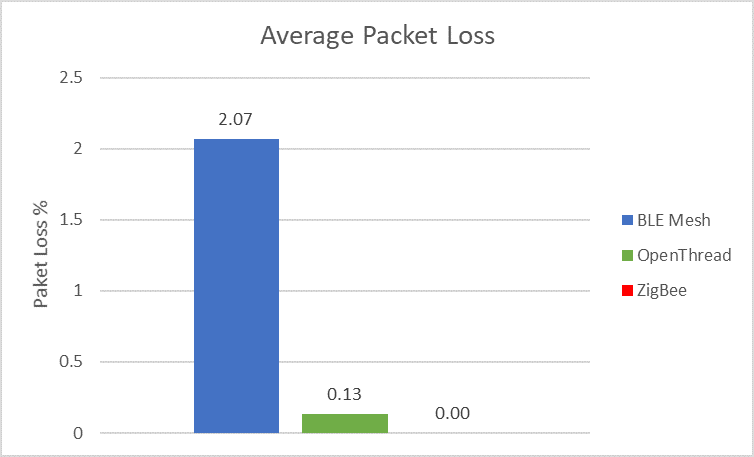
\includegraphics[width=\textwidth]{Average_Packet_Loss.png}
		\caption{Messung 2 Wohnung: Durchschnittlicher Paketverlust}
		\label{fig:DurchschnittlicherPaketverlust}
\end{minipage}
\begin{minipage}[b]{0.49\textwidth}
		\centering
		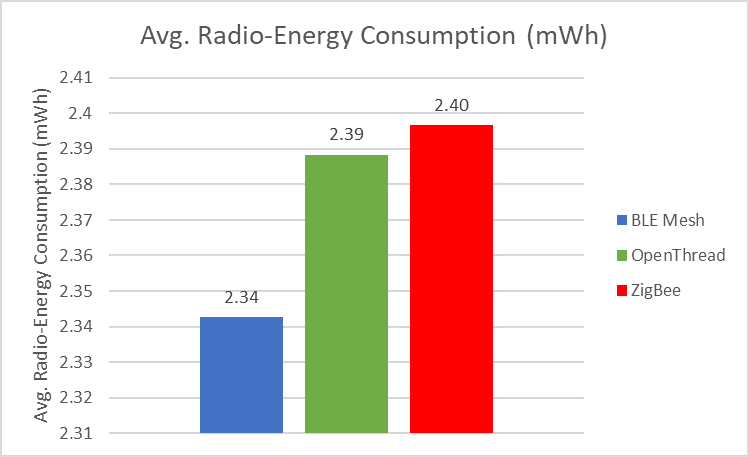
\includegraphics[width=\textwidth]{Average_Radio_Energy_Consumption.png}
		\caption{Messung 2 Wohnung: Durchschnittlicher Energieverbrauch}
		\label{fig:DurchschnittlicherEnergieverbrauch}
\end{minipage}
\end{figure}

Mit dem Diagramm in Abbildung \ref{fig:DurchschnittlicherEnergieverbrauch} wird schliesslich noch der durchschnittliche Energieverbrauch der Protokolle dargestellt.
Dieser ist abgeleitet aus der \textit{Active Radio Time} (siehe Abschnitt \ref{subsubsec:Vergleichswerte}) welche direkt auf dem nRF52840 SoC mit der entsprechenden API ausgelesen werden kann.
Die \textit{Active Radio Time} wurde schliesslich mit dem Strombedarf des SoC's bei definierter Speisesannung von 3V verrechnet.
Gemäss den Angaben in der Tabelle \ref{tab:EigenschaftennRF52840SoC} aus Abschnitt \ref{subsec:SystemonChip} beträgt der Strombedarf bei aktivem Funkmodul im Sendemodus 4.8mA.
Eine solche Berechnung erlaubt einen qualitativen Vergleich des Energiebedarf unter den 3 Protokollen da die Umsetzung auf der gleichen Hardware erfolgte.
Die Werte in der Abbildung \ref{fig:DurchschnittlicherEnergieverbrauch} sind jedoch keine quantitativen Verbrauchswerte und können deshalb nur im Kontext des Vergleichs verwendet werden.
Der Strombedarf sämtlicher Peripherie wurde nicht berücksichtigt da dieser prinzipiell bei allen Protokollen identisch ist.

\begin{figure}[h]
	\centering
	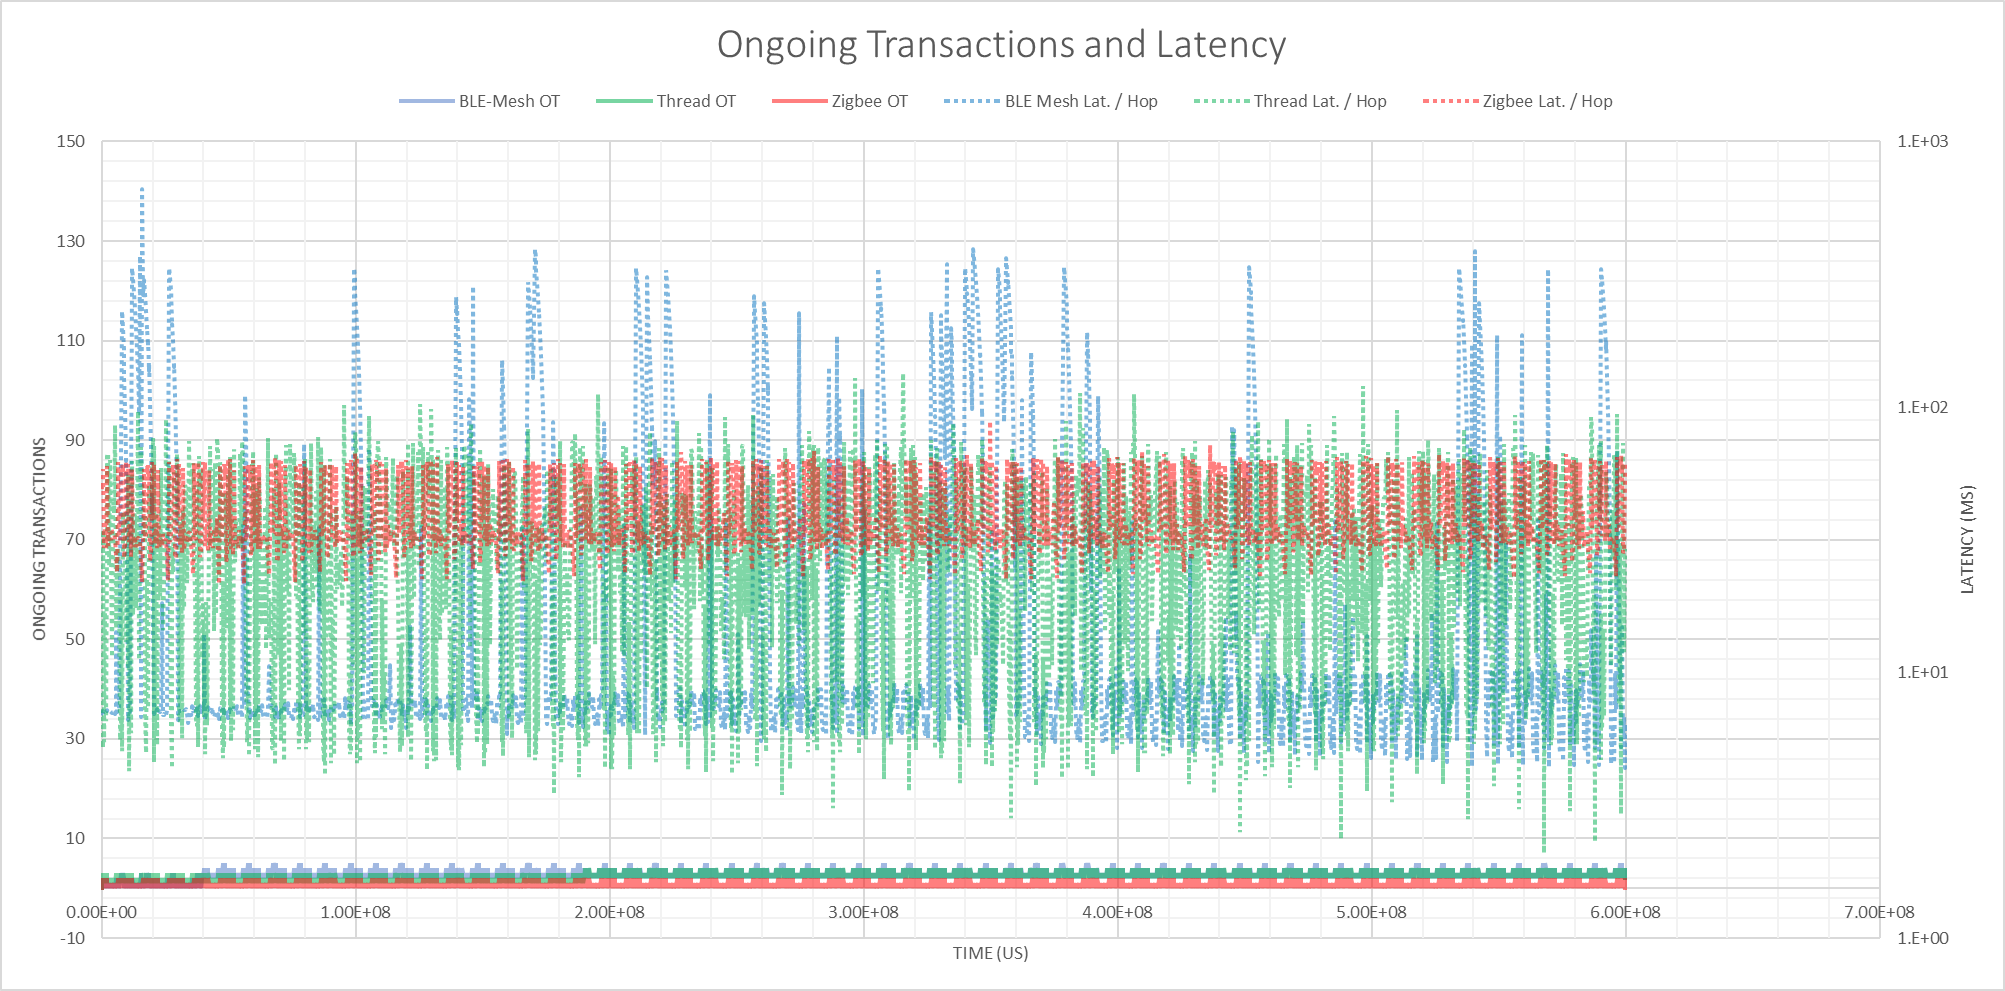
\includegraphics[width=\textwidth]{Ongoing_Transactions_and_Latency.png}
	\caption{Messung 2 Wohnung: Ongoing Transactions und Verlauf der Latenzzeiten über die Messdauer.}
	\label{fig:OngoingTransactions}
\end{figure}

Die letzte Grafik gemäss Abbildung \ref{fig:OngoingTransactions} zeigt den Verlauf der \textit{Ongoing Transactions} sowie der Latenzzeiten über die Gesamtdauer einer Messung.
In diesem Fall beträgt die Dauer 600 Sekunden.
Die Grafik soll einen Eindruck darüber vermitteln, wie die Stacks damit umgehen, wenn vielen Nachrichten zur selben Zeit versendet werden.
Die \textit{Ongoing Transactions} welche als durchgezogene Linien dargestellt sind, zeigen zu welchem Zeitpunkt wie viele Nachrichten in der Übermittlung sind.
Da die Nachrichten in diesem Beispiel sequentiellen versendet werden gibt es nur sehr geringe Ausschläge welche im unteren Bildrand zu sehen sind.
Die logarithmische Darstellung der Latenzzeiten als gestrichelte Linie bestätigt die Beobachtungen die in der Abbildung \ref{fig:VerteilungderLatenzzeiten} bereits gemacht wurden.
Zigbee wie auch Thread weisen einen ziemlich regelmässigen Verlauf der Latenzzeiten auf.
BT Mesh hingegen zeigt starke Ausreisser.

\subsection{Validierung}\label{subsec:Validierung}
Die durchgeführten Messungen haben aussagekräftige Resultate geliefert welche jedoch stark vom gewählten Vorgehen abhängig sind.
Dieses Vorgehen soll nun kritisch überprüft und allfällige Mängel im Konzept sowie der Umsetzung aufgezeigt werden.
Zudem werden systematische Messfehler deklariert.

\paragraph{Large Payload}
Die Messungen 3, 4 und 8 gemäss Tabelle \ref{tab:MessungenMeshBenchmark} welche mit einer grossen Payload durchgeführt wurden, sind nur für Thread und Zigbee aussagekräftig. Der BT Mesh Stack liefert bei diesen Messungen keine brauchbaren Resultate.
Eine Recherche zu diesem Problem hat ergeben, dass durch die Fragmentierung einer 32 Byte Payload die sichere und schnelle Übertragung der Daten nicht mehr gewährleistet werden kann.
\todo[inline]{Referenz auf Artikel wenn vorhanden. Raffi? Ansonsten Text anpassen.}

\paragraph{Zigbee Latency}
Wie bereits im Abschnitt \ref{subsec:Resultate} erwähnt, konnte bei Zigbee die Anzahl Hops die ein Paket passiert hat nicht ausgewertet werden.
Der Forumsbeitrag \href{https://devzone.nordicsemi.com/f/nordic-q-a/63815/zigbee---read-number-of-hops-radius}{\textit{Zigbee - Read number of hops (radius)\footnote{\url{https://devzone.nordicsemi.com/f/nordic-q-a/63815/zigbee---read-number-of-hops-radius}}}} bestätigt, dass der entsprechende Wert mit der verwendeten SDK nicht ausgelesen werden kann.
Als Folge dessen kann schliesslich die Latenzzeit nur als Total über die gesamte Strecke erfasst werden. In der Auswertung verschafft dies BT Mesh und Thread fälschlicherweise einen Vorteil gegenüber Zigbee.
Die Auswertung der totalen Latenzzeit bei allen 3 Protokollen könnte das Problem lösen.
Dies würde jedoch dem Messkonzept widersprechen und wurde deshalb nicht für alle Messungen umgesetzt.
Die Abbildungen \ref{fig:DurchschnittlicheLatenzzeitValidierung} und \ref{fig:DurchschnittlicheLatenzzeitohneHopsValidierung} zeigen den Unterschied am Beispiel der oben analysierten Messung \ref{subsec:Resultate}.
Während links die Latenzzeit pro Hop dargestellt ist, zeigt die rechte Grafik die totale Latenzzeit.
Der Unterschied ist vorallem bei Thread deutlich erkennbar.
Bereits in der Abbildung \ref{fig:VerteilungderLatenzzeiten} ist das Problem zu erkennen.
Die Statistik der Latenzzeiten von Zigbee hat zwei Hauptsäulen bei 40ms und 70ms was auf einen Hop hindeutet.


\begin{figure}[!htbp]
\centering
\begin{minipage}[b]{0.49\textwidth}
		\centering
		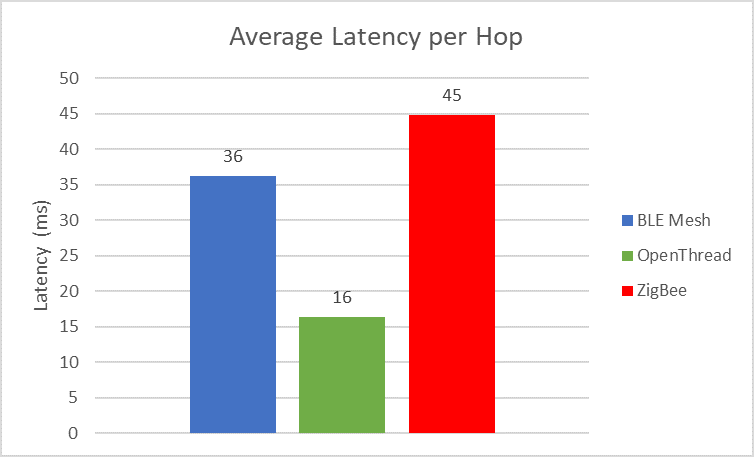
\includegraphics[width=\textwidth]{Average_Latency_per_Hop.png}
		\caption{Durchschnittliche Latenzzeit pro Hop}
		\label{fig:DurchschnittlicheLatenzzeitValidierung}
\end{minipage}
\begin{minipage}[b]{0.49\textwidth}
		\centering
		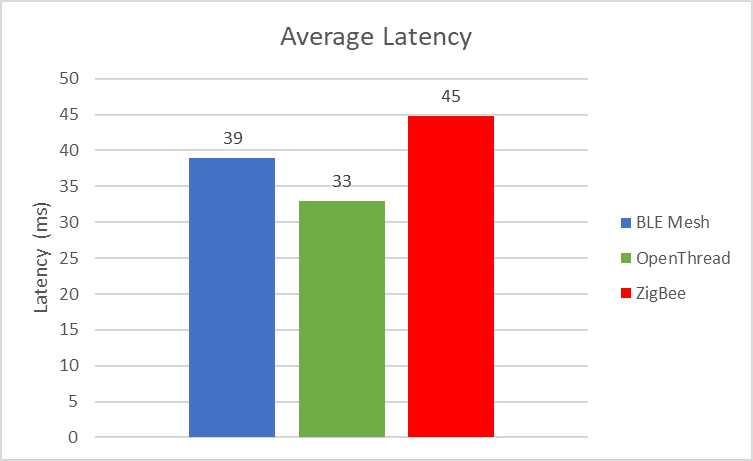
\includegraphics[width=\textwidth]{Average_Latency_without_Hops.png}
		\caption{Durchschnittliche Latenzzeit ohne Berücksichtigung der Hops.}	\label{fig:DurchschnittlicheLatenzzeitohneHopsValidierung}
\end{minipage}
\end{figure}

\paragraph{Nachrichten Dichte}
Bei der Definition der Messreihen \ref{subsec:Messreihe} wurden zu Beginn nur die Messungen 1 bis 6 spezifiziert.
Die Messreihen 7 und 8 kamen erst nachträglich hinzu als festgestellt werden musste, dass die Dichte der Nachrichten für den BT Mesh Stack zu hoch gewählt wurde.
Dieser schien überfordert besonders bei zufälliger Nachrichten Generierung wie im Abschnitt \ref{subsec:TrafficGeneration} beschrieben.
Thread und Zigbee zeigten indes keine Mühe mit der Dichte von 60 Nachrichten in 600 Sekunden pro Node.
Die Resultate der Messungen 7 und 8 haben schliesslich gezeigt, dass die Reduktion der Nachrichtendichte einen positiven Einfluss hat.

\paragraph{Group addressing mode}
Der \textit{Group addressing mode} wurde im Abschnitt \ref{subsec:AllgemeineBenchmarkParameter} für die 3 Protokolle unterschiedlich definiert.
Erste Tests vor den eigentlichen Benchmarks haben gezeigt, dass eine Multicast Adressierung bei Zigbee unbrauchbar ist (siehe Abschnitt \ref{subsubsec:Group addressing mode}).
Deshalb hat man sich entschieden bei Zigbee eine Unicast Adressierung umzusetzen.
Während den Benchmarks musste schliesslich festgestellt werden, dass Zigbee durch diese Änderung ein deutlicher Vorteil erlangt hat.
Besonders auf die Paketverlustrate hat sich die Unicast Adressierung positiv ausgewirkt denn Unicast Nachrichten werden im IEEE 802.15.4 Standard auf MAC Ebene quittiert.
Multicast resp. Broadcast hingegen nicht.

Auch in der Messung Nr. 5 hätte sich die Unicast Adressierung für Zigbee positiv ausgewirkt da die Netzbelastung deutlich geringer gewesen wäre.
 
\paragraph{Durchschnittswerte in den Resultaten}
In den Resultaten \ref{subsec:Resultate} wurden sämtliche Durchschnittswerte als Mittelwerte einschliesslich allfälliger Ausreisser aus den Messwerten gebildet.
Dadurch wurden gewisse Resultate deutlich verfälscht.
In einer neuen Auswertung müsste die Ursache für die einzelnen Ausreisser genauer geklärt werden und diese allenfalls gestrichen werden.


\subsection{Verifizierung}\label{subsec:Verifizierung}
Eine Verifizierung der Messresultate konnte nur anhand des Referenzberichts \textit{AN1142: Mesh Network Performance
Comparison\footnote{\url{https://www.silabs.com/documents/public/application-notes/an1142-mesh-network-performance-comparison.pdf} \cite{silicon_laboratories_inc_an1142_2020}}} von \textit{Silicon Labs} gemacht werden.
Dieser ist auf der Webseite von \textit{Silicon Labs} einsehbar.

Der Vergleich der Messergebnisse hat gezeigt, dass die Grössenordnung der Resultate mit jenen aus dem Bericht von Silicon Labs übereinstimmt.
Selbst die Ausreisser in der Latenzzeit bei BT Mesh liegen im selben Rahmen.
Zudem kann die klare Abhängigkeit der Resultate von der Grösse der Payload bestätigt werden.
Einige Unterschiede sind jedoch in der Verteilung der Latenzzeiten erkennbar.
Im Referenzbericht ist diese in einem Bereich zwischen 20ms und 60ms ziemlich regelmässig während in den Ergebnissen dieser Thesis die Verteilung unregelmässiger daherkommt.






